\documentclass[a4paper,11pt]{article}

%\usepackage[default]{comfortaa}
%\usepackage[T1]{fontenc}



\usepackage[T1]{fontenc}
\usepackage[utf8]{inputenc}
\usepackage{graphicx}
\usepackage{xcolor}
\usepackage{siunitx}

\renewcommand\familydefault{\sfdefault}
\usepackage{tgheros}
\usepackage[defaultmono]{droidmono}

\usepackage{amsmath,amssymb,amsthm,textcomp}
\usepackage{enumerate}
\usepackage{multicol}
\usepackage{tikz}
\usepackage{courier}

\usepackage{geometry}
\geometry{total={210mm,297mm},
left=25mm,right=25mm,%
bindingoffset=0mm, top=20mm,bottom=20mm}

 \usepackage[normalem]{ulem}
\usepackage{booktabs}
\usepackage{url}


\linespread{1.3}

\newcommand{\linia}{\rule{\linewidth}{0.5pt}}

% my own titles
\makeatletter
\renewcommand{\maketitle}{
\begin{center}
\vspace{2ex}
{\huge \textsc{\@title}}
\vspace{1ex}
\\
\linia\\
\@author \hfill \@date

\vspace{4ex}
\end{center}
}
\makeatother
%%%

% custom footers and headers
\usepackage{fancyhdr}
\pagestyle{fancy}
\lhead{}
\chead{}
\rhead{}
\lfoot{Circuitos Lógicos}
\cfoot{}
\rfoot{\thepage}
\renewcommand{\headrulewidth}{0pt}
\renewcommand{\footrulewidth}{0pt}
%

% code listing settings
\usepackage{listings}

\lstset{%
  language = Octave,
  backgroundcolor=\color{white},   
  basicstyle=\footnotesize\ttfamily,       
  breakatwhitespace=false,         
  breaklines=true,                 
  captionpos=b,                   
  commentstyle=\color{gray},    
  deletekeywords={...},           
  escapeinside={\%*}{*)},          
  extendedchars=true,              
  frame=single,                    
  keepspaces=true,                 
  keywordstyle=\color{orange},       
  morekeywords={*,...},            
  numbers=left,                    
  numbersep=5pt,                   
  numberstyle=\footnotesize\color{gray}, 
  rulecolor=\color{black},         
  rulesepcolor=\color{blue},
  showspaces=false,                
  showstringspaces=false,          
  showtabs=false,                  
  stepnumber=2,                    
  stringstyle=\color{orange},    
  tabsize=2,                       
  title=\lstname,
  emphstyle=\bfseries\color{blue}%  style for emph={} 
} 

%% language specific settings:
\lstdefinestyle{Arduino}{%
    language = Octave,
    keywords={void, int boolean},%                 define keywords
    morecomment=[l]{//},%             treat // as comments
    morecomment=[s]{/*}{*/},%         define /* ... */ comments
    emph={HIGH, OUTPUT, LOW}%        keywords to emphasize
}


%%%----------%%%----------%%%----------%%%----------%%%

\begin{document}

\begin{titlepage} % Suppresses displaying the page number on the title page and the subsequent page counts as page 1
	\newcommand{\HRule}{\rule{\linewidth}{0.5mm}} % Defines a new command for horizontal lines, change thickness here
	
	\center % Centre everything on the page
	
	%------------------------------------------------
	%	Headings
	%------------------------------------------------
	
	\textsc{\LARGE Instittuto Tecnológico Autónomo de México}\\[1.5cm] % Main heading such as the name of your university/college
	
	\textsc{\Large Circuitos Lógicos}\\[0.5cm] % Major heading such as course name
	
	\textsc{\large Registros}\\[0.5cm] % Minor heading such as course title
	
	%------------------------------------------------
	%	Title
	%------------------------------------------------
	
	\HRule\\[0.4cm]
	
	{\huge\bfseries Implementación de un Taxímetro de Tarifa Variable}\\[0.4cm] % Title of your document
	
	\HRule\\[1.5cm]
	
	%------------------------------------------------
	%	Author(s)
	%------------------------------------------------
	
	\begin{minipage}{0.4\textwidth}
		\begin{flushleft}
			\large
			\textit{170404}\\
			Silvestre \textsc{González Abreu} % Your name
		\end{flushleft}
	\end{minipage}
	~
	\begin{minipage}{0.4\textwidth}
		\begin{flushright}
			\large
			\textit{173347}\\
			Andrea \textsc{De Anda Kuri} % Supervisor's name
		\end{flushright}
	\end{minipage}
	
	% If you don't want a supervisor, uncomment the two lines below and comment the code above
	%{\large\textit{Author}}\\
	%John \textsc{Smith} % Your name
	
	%------------------------------------------------
	%	Date
	%------------------------------------------------
	
	\vfill\vfill\vfill % Position the date 3/4 down the remaining page
	
	{\large 11 de noviembre, 2019} % Date, change the \today to a set date if you want to be precise
	
	%------------------------------------------------
	%	Logo
	%------------------------------------------------
	
	%\vfill\vfill
	
\includegraphics[width=0.2\textwidth]{itam.jpg}\\[1cm] % Include a department/university logo - this will require the graphicx package
	 
	%----------------------------------------------------------------------------------------
	
	\vfill % Push the date up 1/4 of the remaining page
	
\end{titlepage}

%Aqui va el planteamiento del problema
\section*{Introducción}
En el presente proyecto se tuvo el objetivo de desarrollar un taxímetro capaz de calcular la tarifa de un viaje con base en más de ocho variables de entrada. 
El enfoque principal fue implementarlo de tal manera que fuera sencillo de instalar y desinstalar; no sólo por tratarse de una modificación temporal para los autos utilizados, 
pero también para crear un sistema modular que puede ser compartido por varios autos sin necesidad del uso de herramientas.
    
La mayor parte de las restricciones fueron planteadas como consecuencia de las limitaciones de memoria del sistema utilizado, 
limitaciones de los componentes disponibles o límites definidos para acotar la complejidad de la solución. Algunas de las restricciones fueron definidas en la fase de pruebas al descubrir limitaciones no previstas durante la etapa de planeación, éstas fueron analizadas para encontrar la fuente del problema, y una solución adecuada o, en su defecto, plantear una restricción justificada. 

A lo largo de este proyecto fue necesario tener medidas de seguridad especiales, pues se levantaron los autos utilizados para poder instalar los sensores requeridos y se usaron herramientas como el cautin a altas temperaturas para realizar puntos de soldadura o herramientas de corte. A pesar de que hubo accidentes inesperados en el desarrollo del proyecto, sólo representaron retrasos al itinerario del mismo y riesgos graves para los participantes y colaboradores.

Por último, debido a la naturaleza del problema se requirió de un gran número de pruebas. Inicialmente se probaron de manera individual todos los componentes para descartarlos como posibles fuentes de error en pruebas subsecuentes. En la segunda etapa de pruebas se comprobó la comunicación de la tarjeta Arduino con cada uno de los sensores, displays, botones y módulos usados, nuevamente para descartar fuentes de error. En la tercera etapa se realizaron pruebas del dispositivo terminado pero no instalado en los vehículos, 
es decir, pruebas estáticas para comprobar el código realizado con excepción de la medición de distancia de viaje. Por último, se realizaron las pruebas dinámicas. 
Las primeras de ellas se hicieron en espacios controlados, como estacionamientos y calles poco transitadas a bajas velocidades; y finalmente se pasó a probar velocidades cercanas a los límites de velocidad en vías de acceso controlado.

En resumen, este proyecto consistió en desarrollar el taxímetro con componentes no especializados en el tema, es decir, sin adquirir piezas propias de un taxímetro existente y crear una nueva solución con los conocimientos que tenemos. La gran cantidad de variables de entrada crea una variedad de casos y estados a considerar, por lo que se deben encontrar maneras de agrupar y simplificar el código. Como ya se mencionó, otro factor de complejidad fue la necesidad de instalar de forma no permanente pero segura los sensores necesarios a los vehículos de prueba.


\section*{Planteamiento del problema}
Se plantea el problema de la falta de un dispositivo de instalación sencilla y no permanente para llevar el conteo de la tarifa de un viaje en taxi con el uso de registros y memoria. La mayor parte de los taxímetros actualmente en uso requieren de softwares especializados o modificaciones de hardware para hacer cambios de tarifa y/o cambiar las variables del sistema. Como consecuencia, la solución propuesta es fácil de modificar, pues al estar basada en Arduino se tiene acceso a un software gratuito para alterar los parámetros de cálculo de tarifa. Además, es necesario considerar la posibilidad de añadir los datos de cálculo para más de 30 vehículos y seleccionar el auto en cuestión sin necesidad de usar la computadora. 

Además, se planteó un presupuesto máximo de MXN\$1,500 
para la implementación de la solución generada, 
pues el precio mínimo de un taxímetro comercial se encuentra alrededor de
 MXN\$1,000. Se aumenta el presupuesto sobre el precio comercial, 
 pues se considera que al tratarse de una solución con un mayor número de variables puede requerir una mayor inversión.

 \section*{Restricciones}
 \begin{enumerate}
	\item El taxímetro no se mantiene encendido por más de 45 días de forma contínua, pues para almacenar el tiempo transcurrido desde que se encendió el dispositivo se utilizó una variable de tipo unsigned long. Ésta es una variable de 32 bits (4 bytes) y el tiempo es medido en milisegundos, 
	lo que se traduce un máximo de 4,294,967,295 milisegundos de funcionamiento antes de un desbordo, es decir, 49.71 días.
	\item A lo largo de un viaje pueden agregarse pasajeros (hasta 4), pero el total de pasajeros terminan sus viajes en un mismo punto. Esta restricción se tiene como consecuencia de la cantidad de puertos disponibles en la tarjeta Arduino, pues para permitir la finalización de viaje de forma individual sería necesario un botón adicional y la totalidad de las entradas digitales de la tarjeta se utilizan para la solución presentada. 
	\item No se implementa en el dispositivo la medición de distancia de viaje por medio de GPS debido al costo y a la menor precisión del mismo.
	\item Los vehículos de prueba no deben circular a más de 55 km/h. (Este punto es discutido con mayor detalle en la sección de análisis de resultados)
	\item Se asume que no se puede presionar más de un botón a la vez debido a la elevada velocidad de reloj de 16MHz, por lo que se se registra sólo el primero en ser presionado.
\end{enumerate}

\newpage
\section*{Máquinas de estado}
\begin{figure}[h]
	\centering
	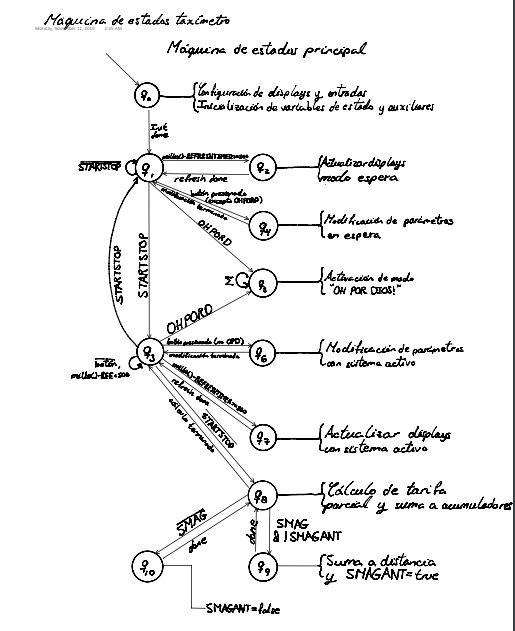
\includegraphics{images/maq1.jpg}
\end{figure}
\newpage
\begin{figure}[h]
	\centering
	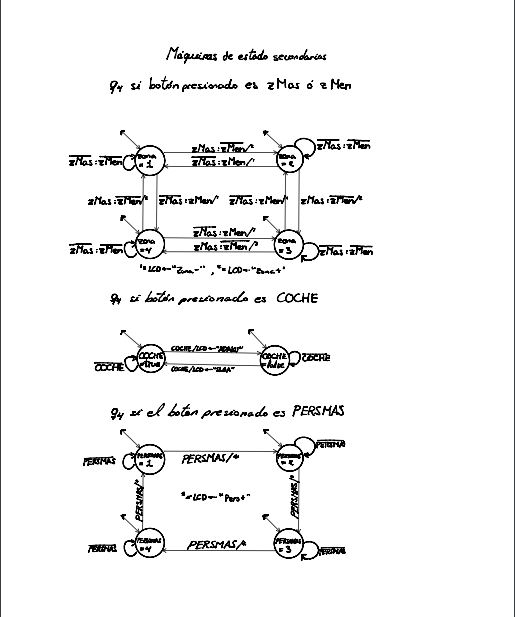
\includegraphics{images/maq2.jpg}
\end{figure}
\newpage
\begin{figure}[h]
	\centering
	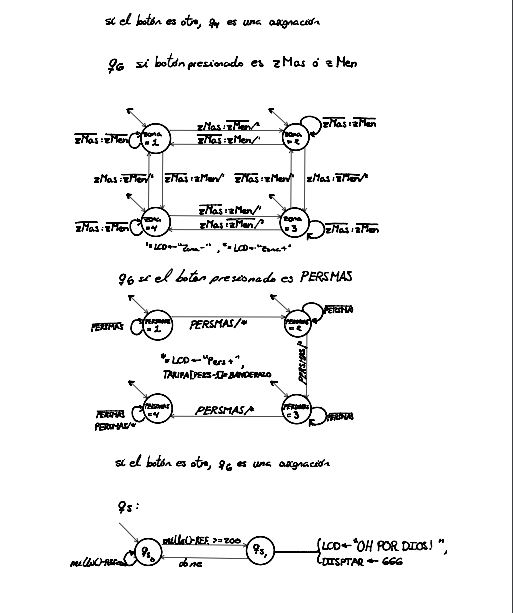
\includegraphics{images/maq3.jpg}
\end{figure}

\section*{Análisis de entradas y salidas}

\subsection*{Tabla de entradas}

\begin{tabular}{ccc}
	Symbol & Descripción & Tipo de variable \\
	STARTSTOP & Botón de activación y desactivación del sistema & Entrada (bit) \\
	ZMAS & Botón para aumentar la zona de viaje & Entrada (bit) \\
	ZMEN & Botón para reducir la zona de viaje & Entrada (bit) \\
	COCHE & Botón para alternar el coche en uso entre los almacenados & Entrada (bit) \\
	PERSMAS & Botón para aumentar en uno la variable de estado PERSONAS & Entrada (bit) \\
	PARAMAS & Botón para aumentar el número de paradas & Entrada (bit) \\
	DIAMAS & Botón para aumentar el día de la semana & Entrada (bit) \\
	HORAMAS & Botón para aumentar 20 minutos a la hora actual del sistema & Entrada (bit) \\
	HORAMEN & Botón para restar 20 minutos a la hora actual del sistema & Entrada (bit) \\
	SMAG & Sensor magnético para detección de giro de las ruedas & Entrada (bit) \\
	OHPORD & Botón para activar el modo OHPORDIOS & Entrada (bit) \\
	DISPTAR & Número entero de 4 dígitos a mostrar en los 7 segmentos & Salida (int) \\
	DISTANCIA & Cantidad de kilómetros recorridos & Salida (double) \\
	ACTIVESTR & Parte del mensaje a desplegar en LCD & Salida (String) \\
	TARIFA[4] & Arreglo para almacenar las tarifas por persona & Salida (double[4]) \\
	LCD & Texto a desplegar en la pantalla LCD & Salida (String) \\
	ACTIVE & Indica si el taxímetro está corriendo actualmente & Estado (bool) \\
	ISCOCHE & Indica si el vehículo seleccionado es auto o camioneta & Estado (bool) \\
	ZONA & Indica la zona seleccionada actual & Estado (int) \\
	PERSONAS & Indica el número de personas seleccionado & Estado (int) \\
	RTC & Módulo de fecha y hora actual & Estado (RtcDateTime) \\
	MODODIOS & Indica si actualmente está activado el modo OHPORDIOS & Estado (bool) \\
	\end{tabular}

\newpage
\subsection*{Tabla de salidas}

\begin{figure}[h]
	\centering
	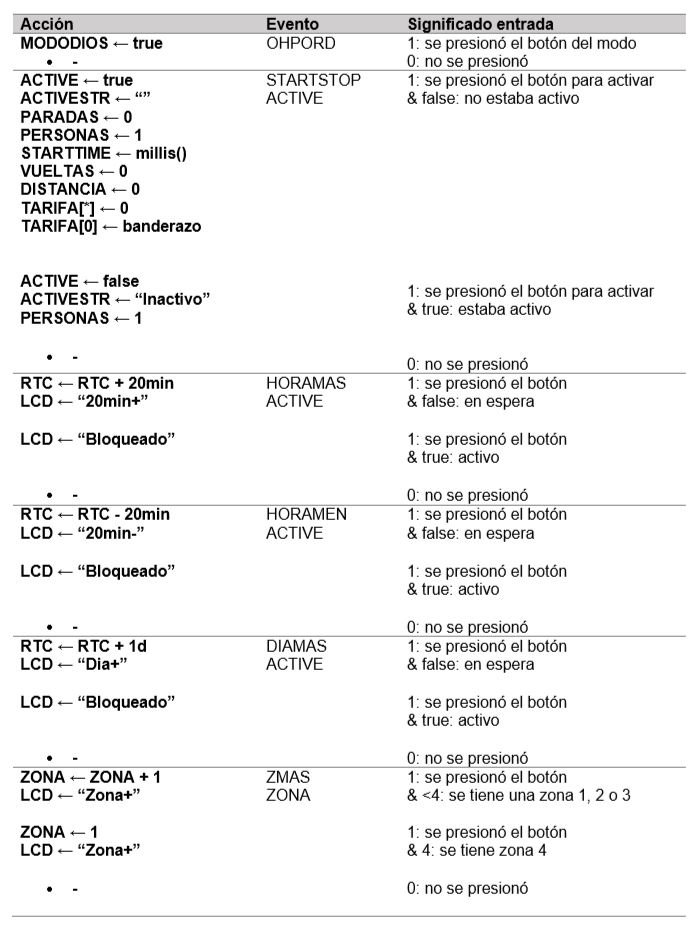
\includegraphics{images/tabla1.jpg}
	\end{figure}
	\newpage
\begin{figure}[h]
	\centering
	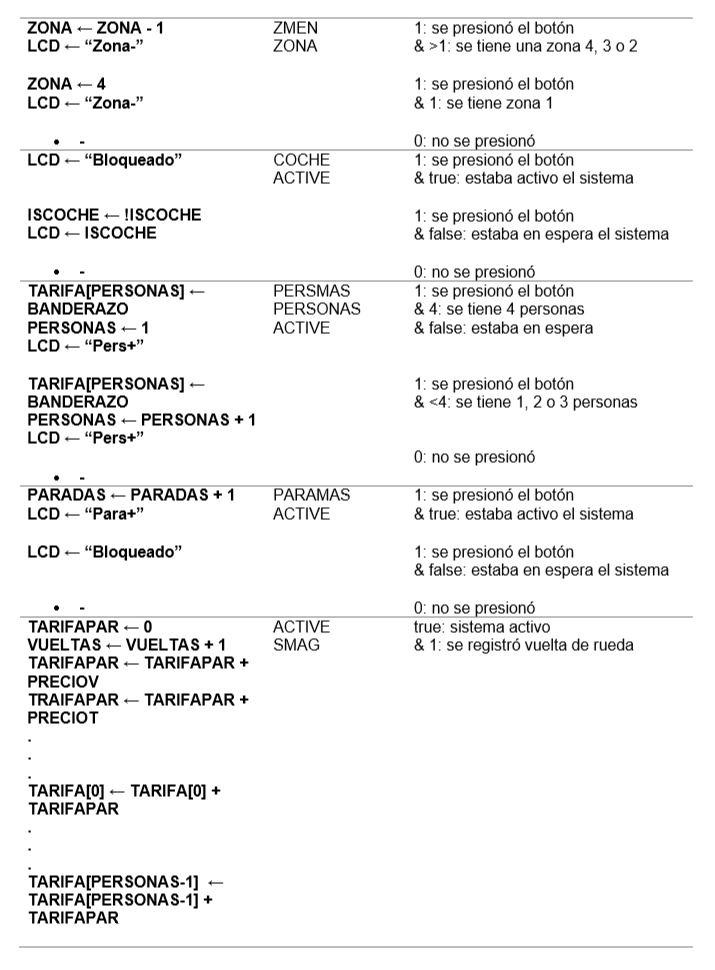
\includegraphics{images/tabla2.jpg}
	\end{figure}

	\newpage
	\begin{figure}[h]
		\centering
		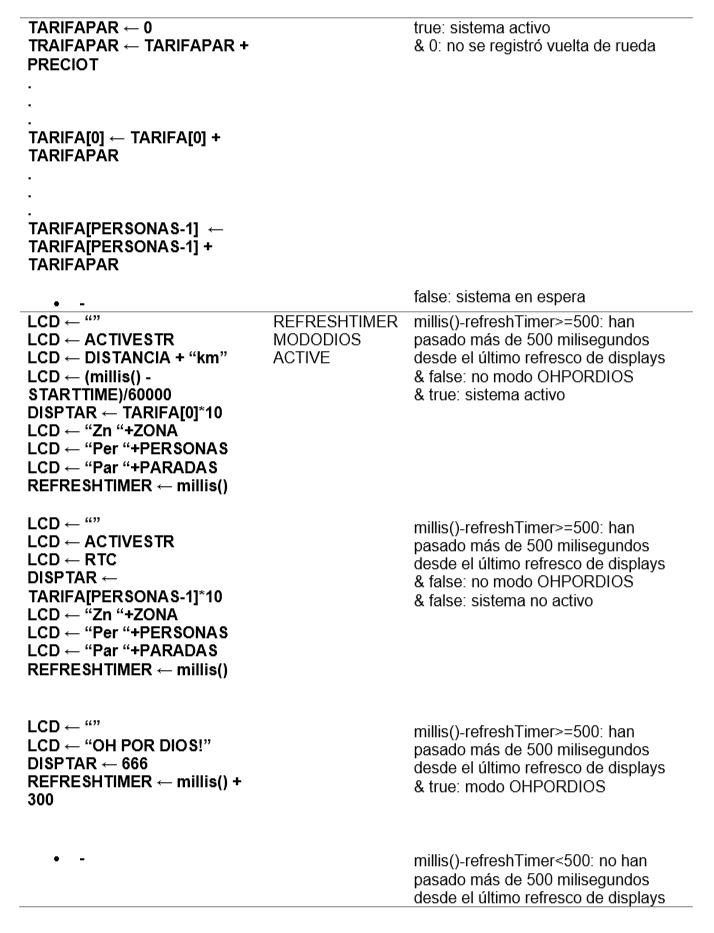
\includegraphics{images/tabla3.jpg}
		\end{figure}
	


\section*{Resultados}

\subsection*{Material}
\begin{itemize}
	\item 1 tarjeta Arduino Mega
	\item 1 módulo RTC para Arduino
	\item 1 pantalla LCD de 16x2
	\item 1 display de 7 segmentos de 4 dígitos
	\item 1 potenciómetro de \SI{5}{\ohm}
	\item 10 resistores de \SI{10000}{\ohm}
	\item 4 resistor de \SI{330}{\ohm}
	\item 1 resistor de \SI{220}{\ohm}
	\item 10 push buttons
	\item 2 sensores magnéticos
	\item 1 protoboard pequeño
	\item 1 tabla de madera de 40x40cm de 3mm de espesor 
	\item 1 montura de succión para parabrisas 
	\item 1 conector para encendedor de auto
	\item 1 plug para Arduino
	\item 4 imanes de neodimio de 1cm de diametro
	\item ~30 jumpers hembra-macho
	\item ~20 jumpers macho-macho
	\item ~10 metros de alambre calibre 22
	\item Cinta de aislar
	\item Cinta doble cara
	\item Soldadura de plomo/estaño
	\item 2 autos	
\end{itemize}

\begin{figure}[h]
\centering
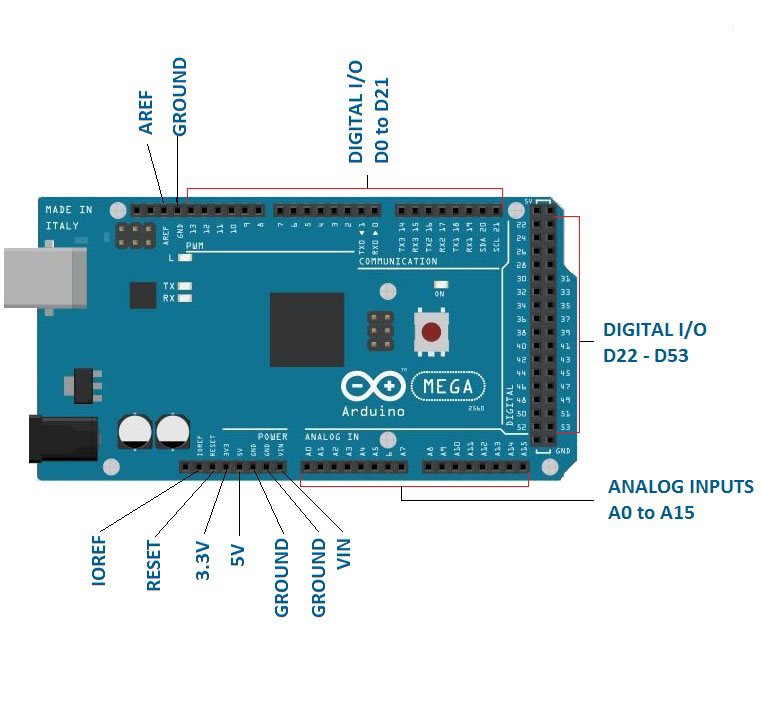
\includegraphics[width=8cm]{images/Arduino.jpg}
\caption{Arguino Mega}
\end{figure}

\newpage
\subsection*{Desarrollo del circuito}
En la siguiente figura se puede ver el circuito final, para desarrollarlo fue necesario planificar adecuadamente 
pues de otra manera los puertos del Arduino Mega no hubieran sido suficientes.

\begin{figure}[h]
	\centering
	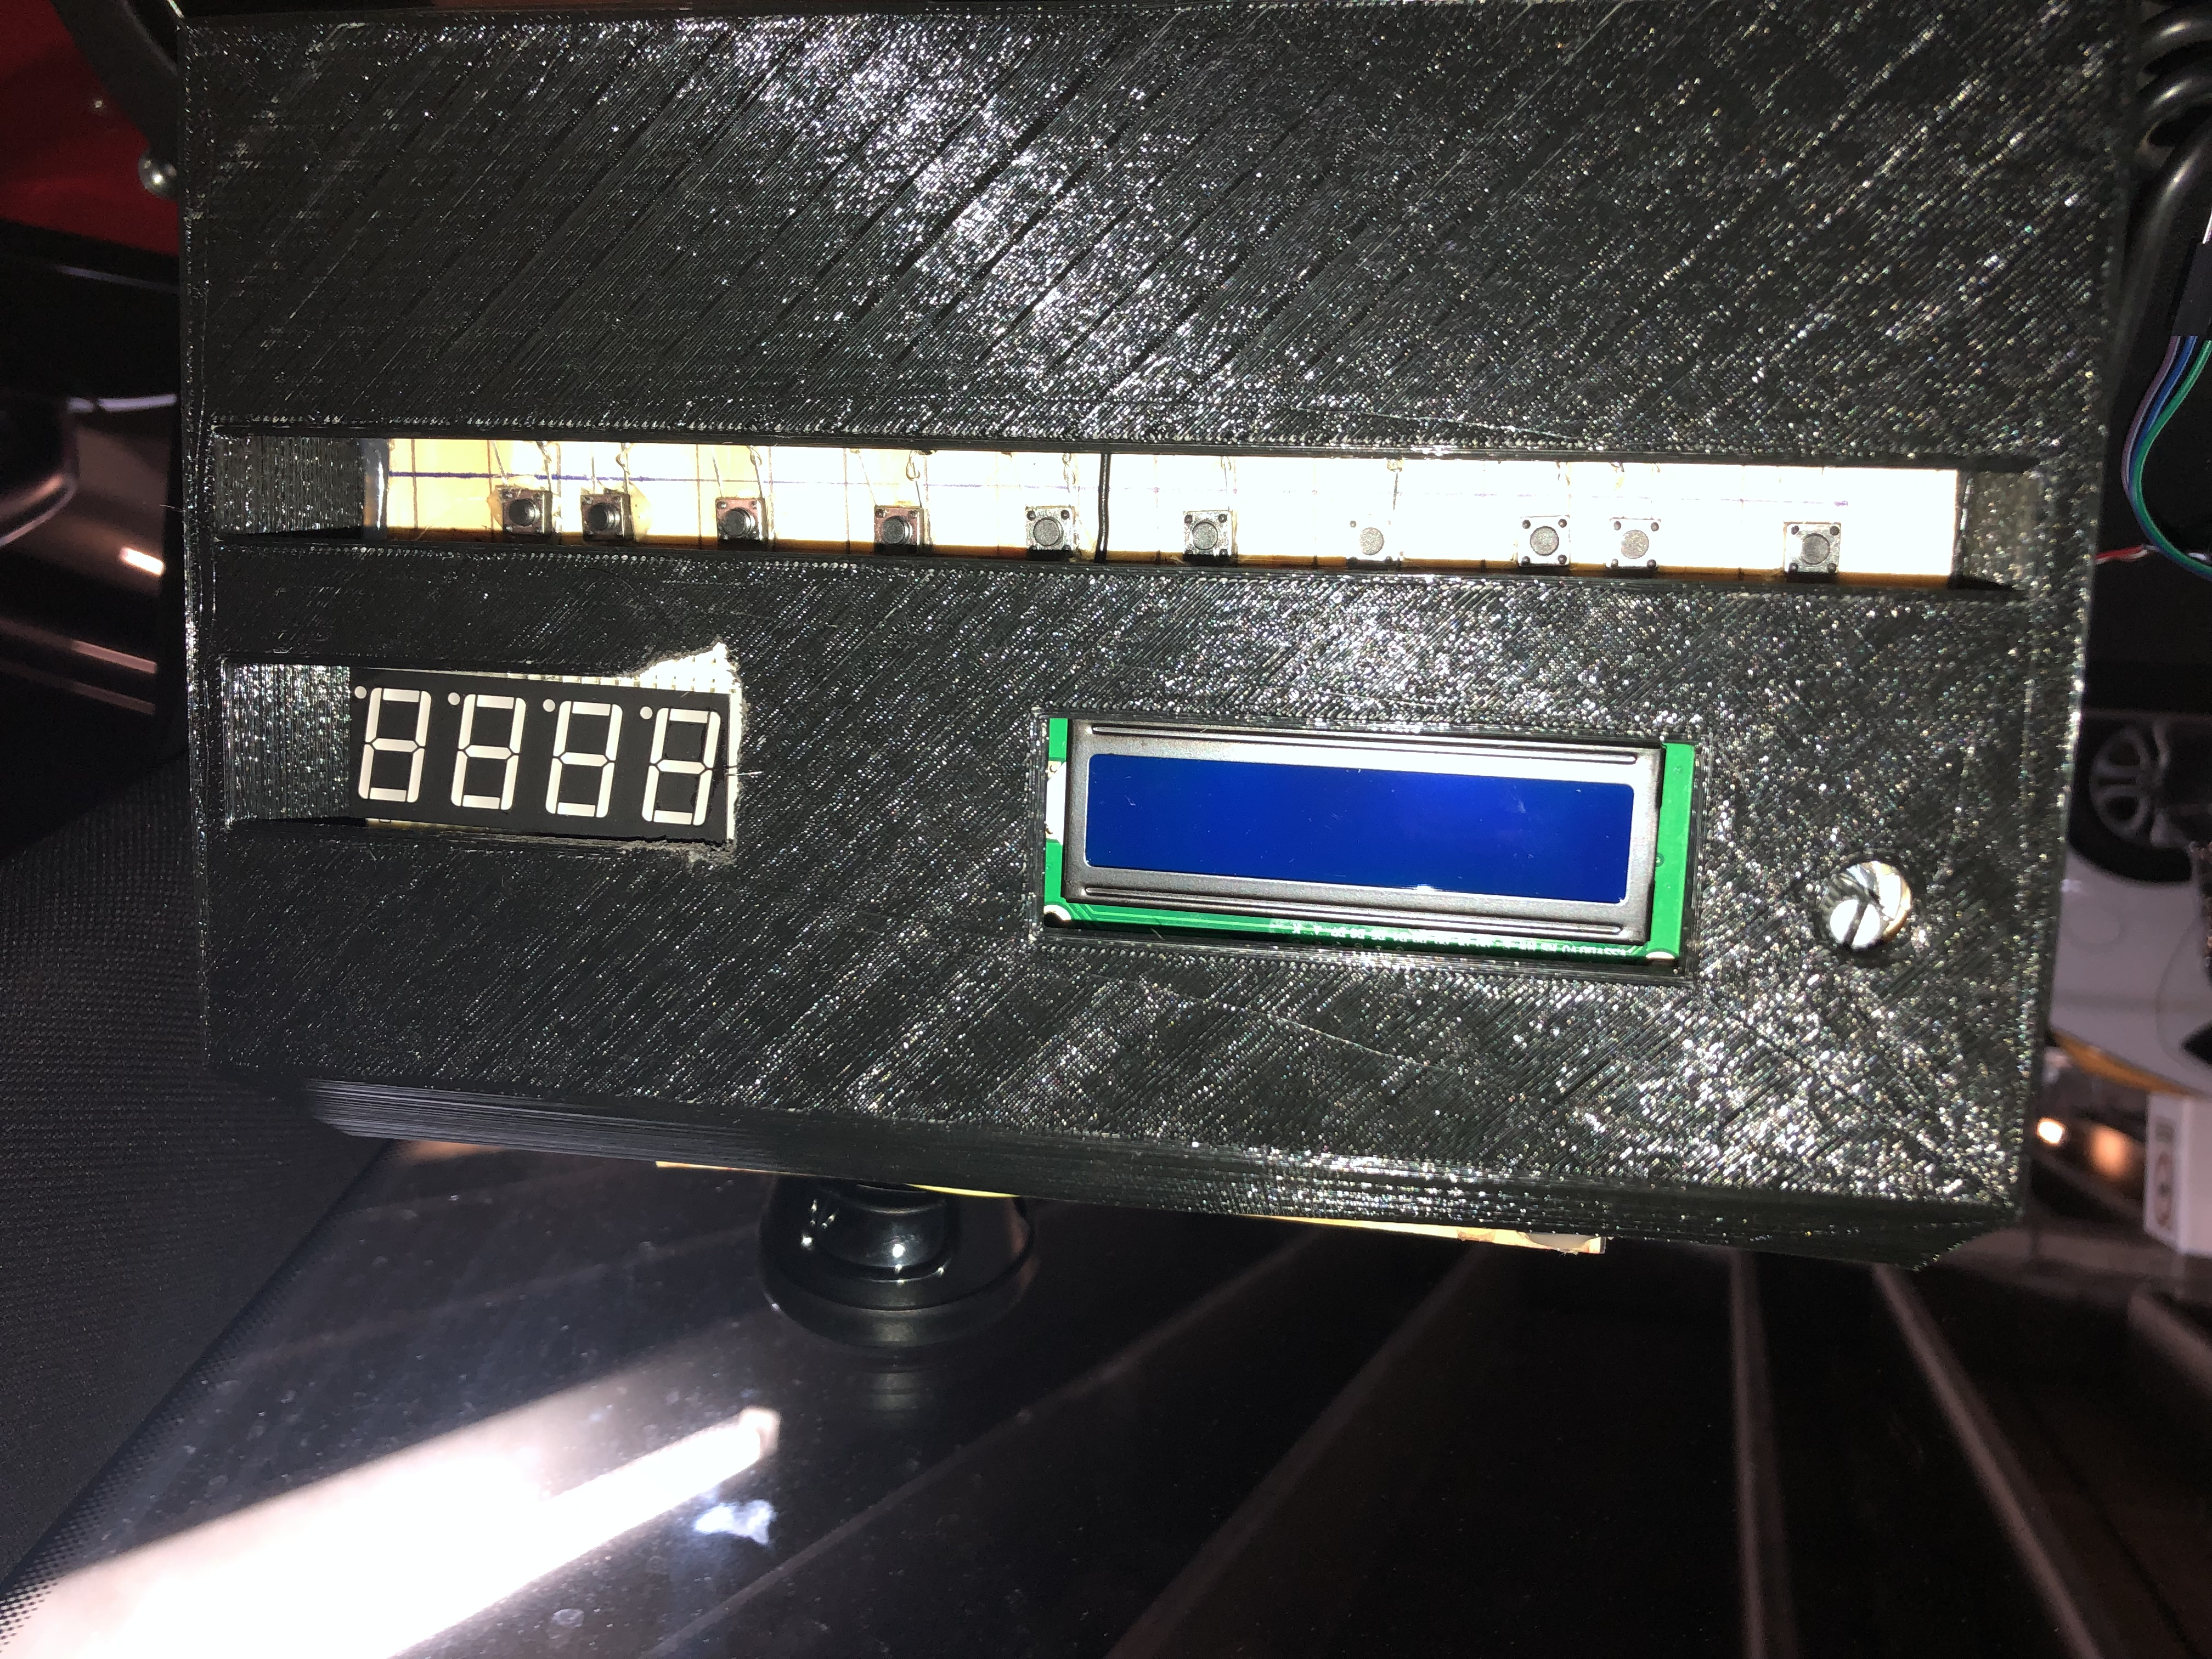
\includegraphics[width=10cm]{images/taximetro.jpg}
	\caption{Vista frontal del taxímetro}
\end{figure}
Para la implementación del circuito se utilizó un Arduino Mega $($código se encuentra abajo$)$, al que se conectaron 
10 push bottons, un sensor magnético y un reloj. Los push buttons fueron conectados a un puerto diferente cada uno, 
pero se conectaron los 10 a una misma tierra y un mismo VCC. Además, los sensores magnéticos están conectados a
la tolva posterior del lado del copiloto de los coches y los imanes de neodimio se encuentran pegados a la parte interior del rin.

Para instalar el taximetro en los autos de prueba se utilizó la montura de succión para parabrisas y se alimentó el circuito por medio 
del puerto para encenderdor del auto. Éste proveé 12V, y aunque el Arduino podría ser alimentado directamente por este voltaje, 
se usó un adaptador para bajar el voltaje a 6V.



\begin{figure}[h]
	\centering
	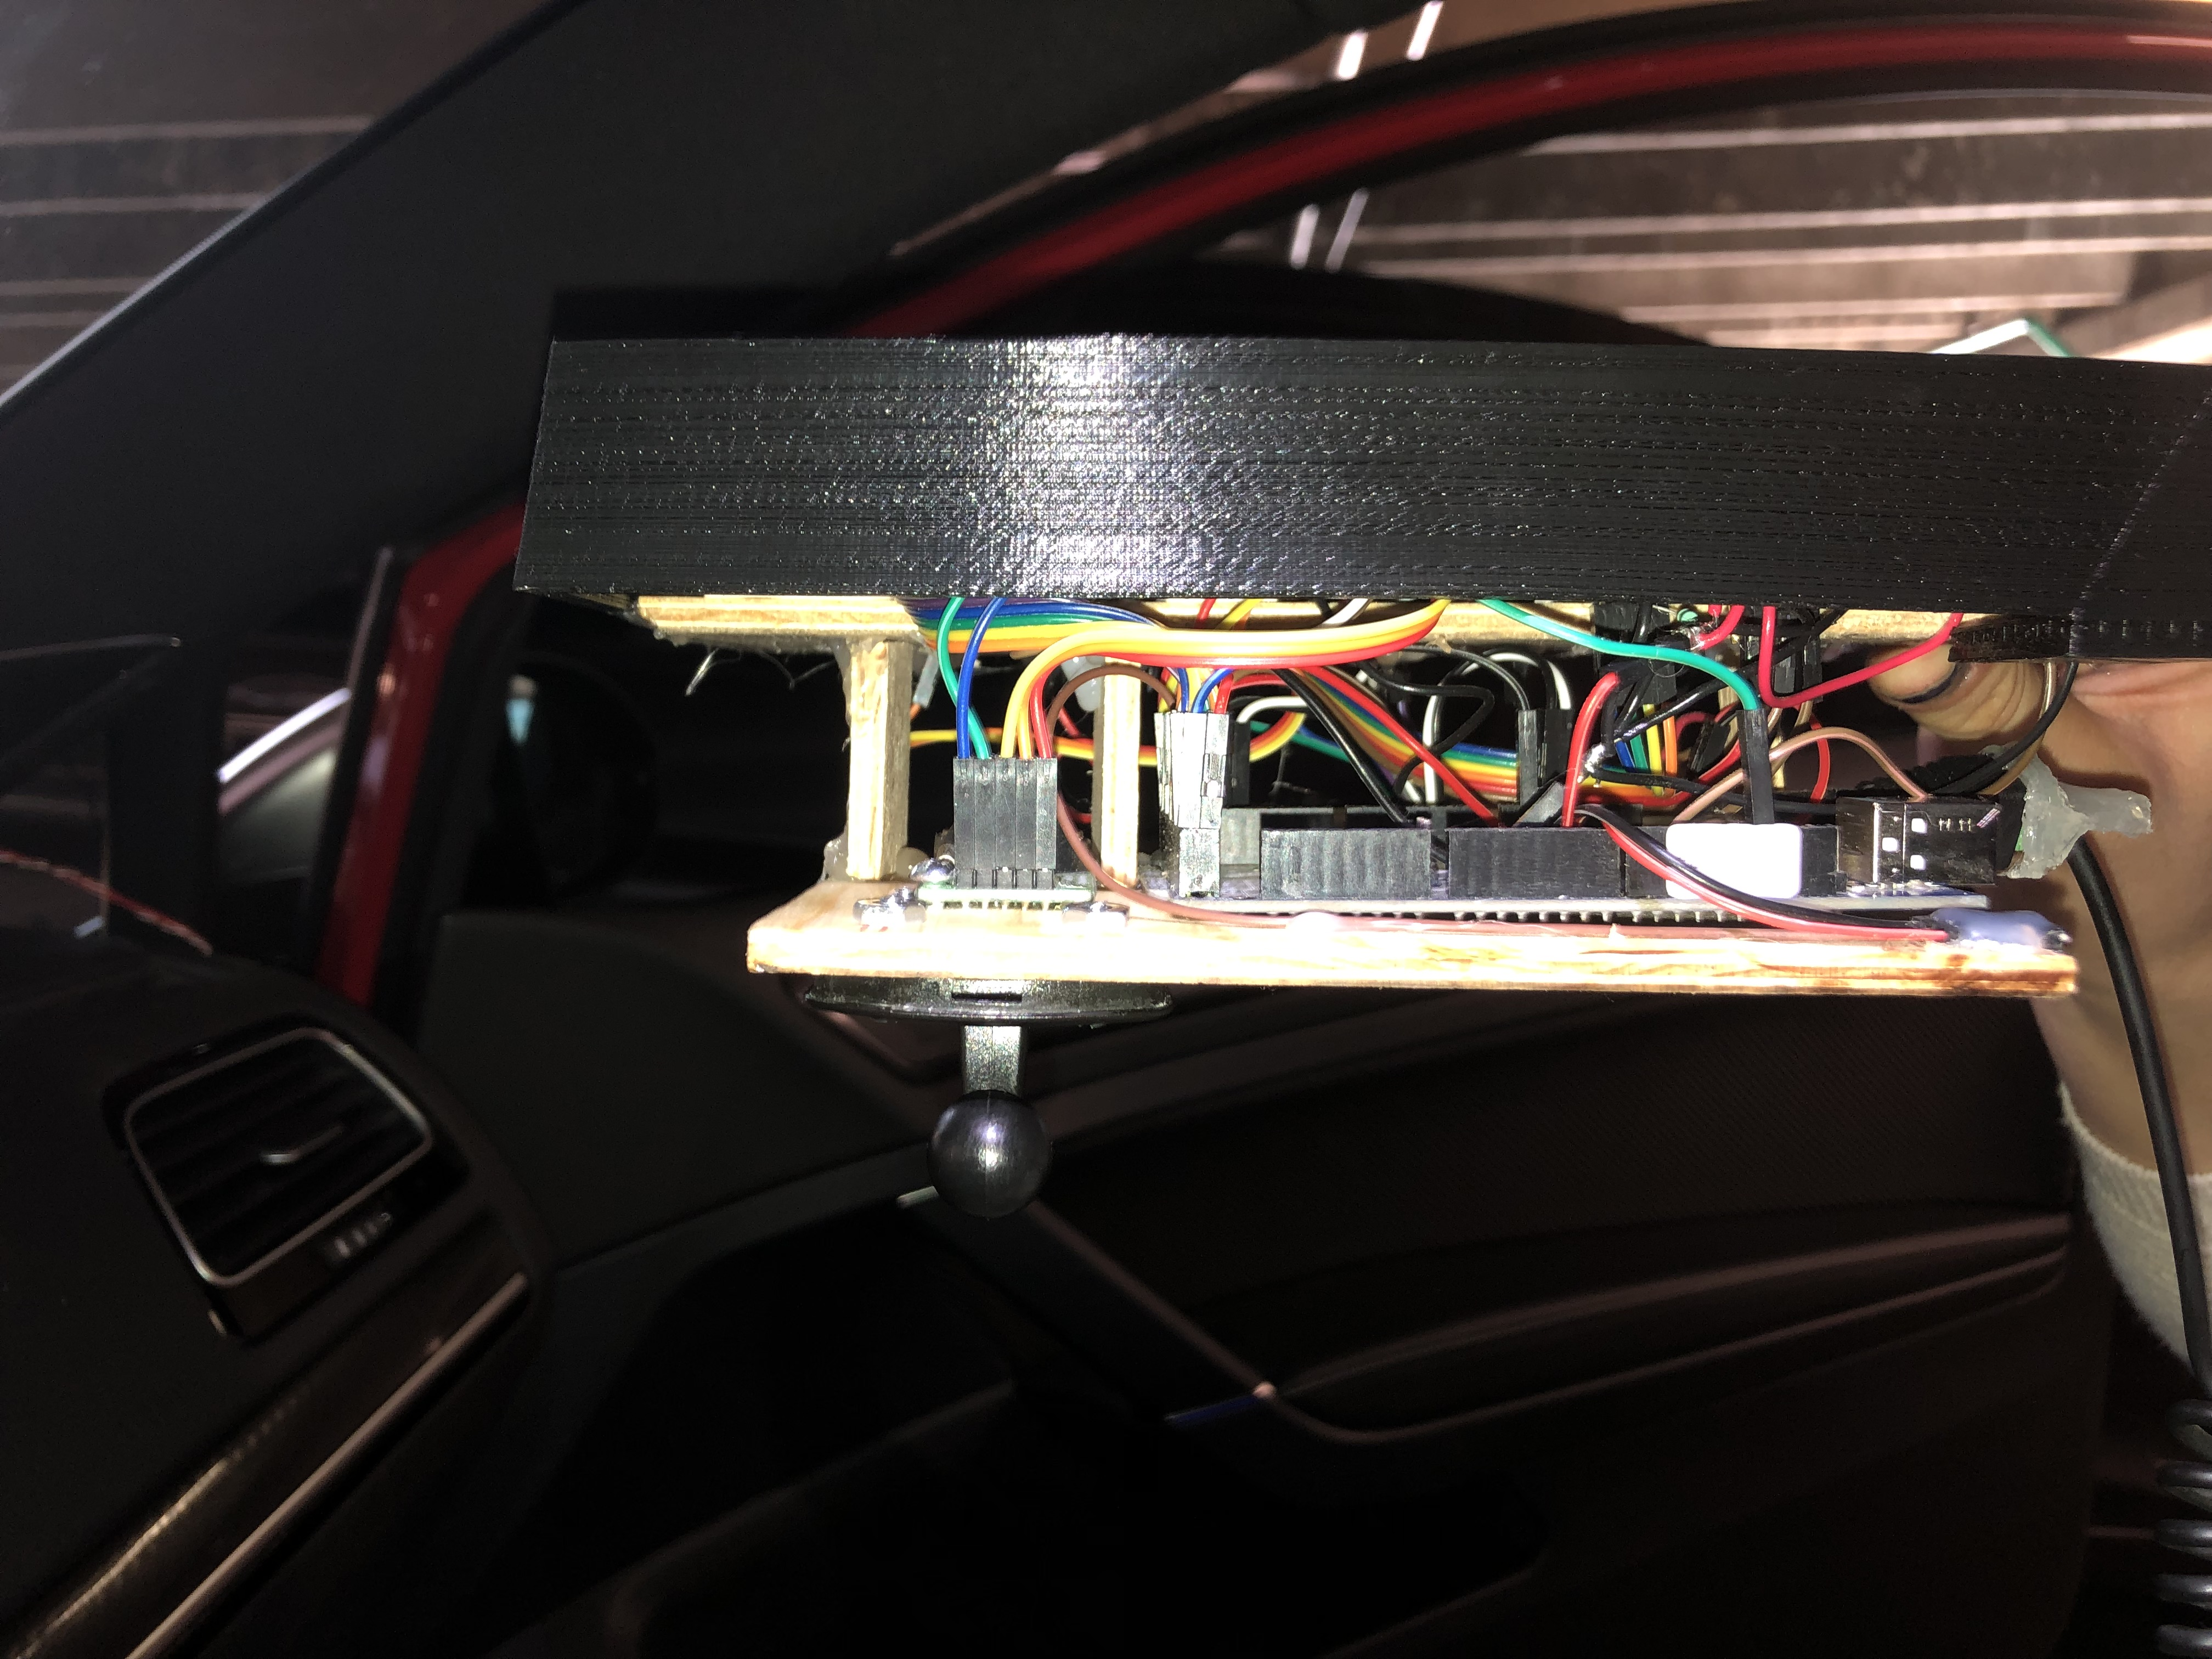
\includegraphics[width=10cm]{images/vista.jpg}
	\caption{Cableado del circuito}
\end{figure}

\newpage
\subsection*{Código desarrollado para la implementación del taxímetro}

\lstinputlisting[style=Arduino]{tarifador_V1/tarifador_V1.ino}

\section*{Análisis de resultados}
En la mayor parte de las pruebas realizadas se obtuvieron los resultados esperados, 
pues la tarifa y los parámetros mostrados corresponden con los cálculos realizados y con los 
valores reales de tiempo y distancia. Esta correspondencia se cumple para las primeras tres etapas de 
pruebas y la primera fase de la cuarta etapa. En la última fase de pruebas se realizaron pruebas a 
velocidades por encima de 70 km/h, en las que se pudo observar un valor de distancia registrado 
entre 10\% y 20\% menor al valor real. 
\\
Este error se puede ocasionar por diversos factores y a continuación se discuten junto con 
las posibles soluciones. En primer lugar, se puede deber a que el sensor magnético no tiene 
suficiente tiempo para detectar el paso del imán. Esto podría solucionarse al colocar el arreglo
 de sensor-imán más cerca del centro de la rueda, lo que reduciría la velocidad del imán con respecto 
 al sensor sin modificar el número de vueltas registradas. En segundo lugar puede ser consecuencia de 
 interferencia entre los alambres del sensor, pues recorren una distancia relativamente larga y a altas 
 velocidades el valor del sensor cambia rápidamente, lo que se podría corregir separando físicamente los 
alambres. Por último, puede deberse a un error inherente a la utilización de un sensor magnético; 
este problema podría ser corregido haciendo uso del puerto OBDII del auto para obtener datos de
 velocidad y revoluciones del motor. Esta solución fue considerada, pero se descartó debido al aumento 
 considerable de costos por el adaptador necesario para la comunicación OBDII-Arduino.
 
 

\section*{Conclusión}
El proyecto realizado presentó una serie de retos inesperados de todas la áreas involucradas, pues antes de empezar con el desarrollo tangible se tuvo que planear a detalle el material necesario y el itinerario de trabajo. Esto fue de gran importancia pues los puertos digitales del Arduino Mega fueron aprovechados en su totalidad, lo que puede verse tanto como una limitante de hardware o como una optimización de los recursos disponibles. 

    Más adelante se tuvieron que resolver problemas propios de electrónica, pues se planearon las redes de entradas y salidas, así como el cableado de los displays utilizados y el cálculo de los resistores asociados. Posterior a la etapa de cableado y diseño físico de la caja impresa en 3D (modelada en NX), se pasó a la implementación del código para resolver el problema, en la que se consultaron ampliamente las referencias de los componentes utilizados y se aprendió en el proceso. Por último, al instalar el sistema en los autos de prueba se tuvieron que considerar no sólo las partes móviles, pero también las fuentes de calor como el sistema de frenado; y también se planteó el problema de trabajar de manera segura debajo de un vehículo.

    En general se pudo aprender de este proyecto más allá de los temas de la materia de Circuitos Lógicos con experiencias y problemas tangibles. Consideramos que fue de gran utilidad para poner a prueba la capacidad de resolver problemas nuevos con los conocimientos adquiridos hasta el momento y unos cuantos más que fue necesario investigar.

\section*{Referencias}

\begin{enumerate}
	\item Knap.at. $($2019$)$. $[$online$]$ Available at: \url{http://www.knap.at/datenblaetter/led/} $[$Accessed 11 Nov. 2019$]$
	\item SURTR TECHNOLOGY. $($2019$)$. How to simply use DS1302 RTC module with Arduino board and LCD screen. $[$online$]$ Available at: \url{https://surtrtech.com/2018/01/27/how-to-simply-use-ds1302-rtc-module-with-arduino-board-and-lcd-screen/} $[$Accessed 11 Nov. 2019$]$.
	\item Pattabiraman, K. $($2019$)$. How to Set up 7-Segment Displays on the Arduino - Circuit Basics. $[$online$]$ Circuit Basics. Available at: \url{http://www.circuitbasics.com/arduino-7-segment-display-tutorial/} $[$Accessed 11 Nov. 2019$]$.
	\item Forward.com.au. $($2019$)$. How to code Timers and Delays in Arduino. $[$online$]$ Available at: \url{https://www.forward.com.au/pfod/ArduinoProgramming/TimingDelaysInArduino.html} $[$Accessed 11 Nov. 2019$]$.
	\item Circuitstoday.com. $($2019$)$. $[$online$]$ Available at: \url{http://www.circuitstoday.com/wp-content/uploads/2014/06/interfacing-LCD-to-arduino.png} $[$Accessed 11 Nov. 2019$]$.
	\item Arduino.cc. $($2019$)$. Arduino - HelloWorld. $[$online$]$ Available at: \url{https://www.arduino.cc/en/Tutorial/HelloWorld} $[$Accessed 11 Nov. 2019$]$.
	\item GitHub. $($2019$)$. Makuna/Rtc. $[$online$]$ Available at: \url{https://github.com/Makuna/Rtc/wiki/RtcDateTime-object} $[$Accessed 11 Nov. 2019$]$.
	\item Arduino.cc. $($2019$)$. Arduino Reference. $[$online$]$ Available at: \url{https://www.arduino.cc/reference/en/#page-title} $[$Accessed 11 Nov. 2019$]$.
	

\end{enumerate}
	Adicionalmente, se puede consultar el código completo en \url{https://github.com/adeandak/taximetro}
\end{document}
